\chapter{Link Loss vs Noise}
\label{ch:link-loss-vs-noise}

\begin{nontechnical}
\textbf{Link loss vs noise is like the difference between someone whispering (weak signal) vs shouting in a loud room (noise interference)---two different problems!}

\textbf{Link Loss} - Signal gets weaker:
\begin{itemize}
\item \textbf{What it is}: Your WiFi router is far away, so signal is weak by the time it reaches you
\item \textbf{Analogy}: Shouting across a football field---your voice spreads out and gets quieter
\item \textbf{Predictable}: Same distance = same loss every time
\item \textbf{Solution}: Move closer, use bigger antenna, increase transmit power
\end{itemize}

\textbf{Examples of link loss}:
\begin{itemize}
\item \textbf{WiFi}: 50 meters away = 10,000$\times$ weaker signal
\item \textbf{Cell phone}: Far from tower = fewer bars
\item \textbf{Satellite}: Space is far! Signal arrives incredibly weak
\end{itemize}

\textbf{Noise} - Random interference added:
\begin{itemize}
\item \textbf{What it is}: Random electrical static from electronics, thermal energy, cosmic rays
\item \textbf{Analogy}: Trying to hear someone whisper in a noisy restaurant---extra sound covers the signal
\item \textbf{Random}: Unpredictable, changes moment-to-moment
\item \textbf{Solution}: Can't remove it! Must send stronger signal or use error correction
\end{itemize}

\textbf{Examples of noise}:
\begin{itemize}
\item \textbf{Bluetooth stuttering near microwave}: Microwave adds noise
\item \textbf{AM radio crackle}: Thunderstorms add noise
\item \textbf{TV static}: No signal? You're seeing pure noise!
\end{itemize}

\textbf{Key difference}:
\begin{itemize}
\item \textbf{Link loss}: Makes signal weaker (deterministic, predictable)
\item \textbf{Noise}: Adds random garbage on top (random, unpredictable)
\item \textbf{Both hurt you}: Weak signal (loss) covered by noise = errors!
\end{itemize}

\textbf{The engineering ratio: SNR (Signal-to-Noise Ratio)}
\begin{itemize}
\item Strong signal + low noise = high SNR = perfect communication
\item Weak signal (loss) + high noise = low SNR = errors everywhere
\end{itemize}

\textbf{When you see it}: Your phone shows ``5 bars'' (link loss is low) but internet is slow (noise is high from interference).
\end{nontechnical}

\section{Overview}

In a real communication system, the received signal is degraded by \textbf{two distinct mechanisms}: link loss and additive noise.

\begin{keyconcept}
Link loss and noise are \textbf{fundamentally different} phenomena. Link loss deterministically \textbf{attenuates} the signal power, while noise \textbf{adds} random fluctuations. Both must be understood separately to design reliable communication systems, as they require different mitigation strategies.
\end{keyconcept}

\section{Mathematical Description}

\subsection{Link Loss (Path Loss)}\label{link-loss-path-loss}

\textbf{Link Loss} represents the reduction in signal power as it
travels from transmitter to receiver.

\subsubsection{Characteristics}\label{characteristics}

\begin{itemize}
\tightlist
\item
  \textbf{Deterministic}: Same loss every time (for a given scenario)
\item
  \textbf{Multiplicative}: Scales the entire signal uniformly
\item
  \textbf{Predictable}: Can be calculated from path distance, frequency,
  antenna gains
\end{itemize}

\subsubsection{Sources}\label{sources}

\begin{itemize}
\tightlist
\item
  Free-space path loss
\item
  Antenna gains (TX and RX)
\item
  Cable losses
\item
  Atmospheric absorption
\item
  Rain attenuation
\end{itemize}

\subsubsection{Mathematical Model}\label{mathematical-model}

In linear scale, link loss is a multiplicative attenuation:
\begin{equation}
P_{\text{received}} = \frac{P_{\text{transmitted}}}{L}
\end{equation}
where:
\begin{itemize}
\item $P_{\text{received}}$ = received signal power (watts)
\item $P_{\text{transmitted}}$ = transmitted signal power (watts)
\item $L$ = link loss factor (dimensionless, $L \geq 1$)
\end{itemize}

In logarithmic (dB) scale, link loss becomes a subtraction:
\begin{equation}
P_{\text{received}} [\text{dBm}] = P_{\text{transmitted}} [\text{dBm}] - L_{\text{dB}}
\end{equation}
where:
\begin{itemize}
\item $L_{\text{dB}} = 10\log_{10}(L)$ = link loss in decibels
\end{itemize}

\subsubsection{Link Budget Components}

A complete link budget accounts for all gains and losses in the signal path:

\begin{center}
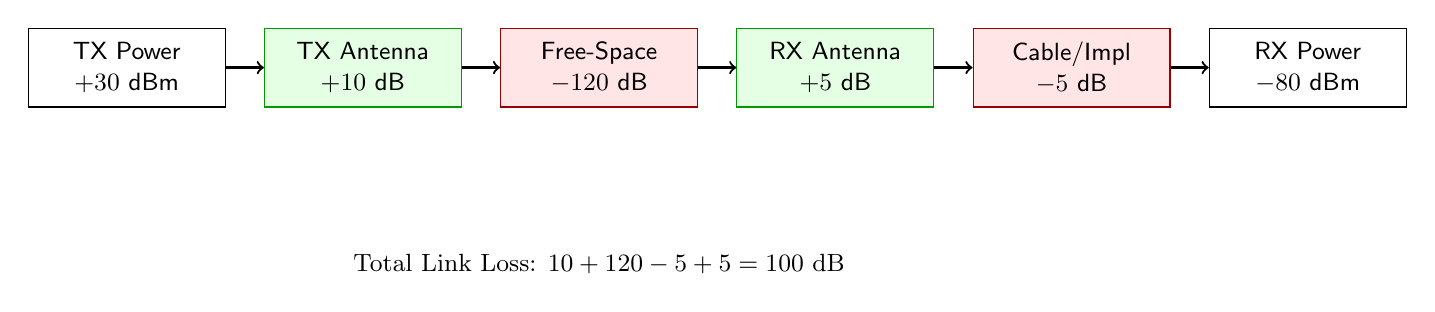
\begin{tikzpicture}[
  node distance=1.8cm,
  block/.style={rectangle, draw, minimum width=2.5cm, minimum height=1cm, font=\sffamily\small, align=center},
  gain/.style={rectangle, draw=green!60!black, fill=green!10, minimum width=2.5cm, minimum height=1cm, font=\sffamily\small, align=center},
  loss/.style={rectangle, draw=red!60!black, fill=red!10, minimum width=2.5cm, minimum height=1cm, font=\sffamily\small, align=center}
]

\node[block] (tx) {TX Power\\$+30$ dBm};
\node[gain, right of=tx, node distance=3cm] (txant) {TX Antenna\\$+10$ dB};
\node[loss, right of=txant, node distance=3cm] (fspl) {Free-Space\\$-120$ dB};
\node[gain, right of=fspl, node distance=3cm] (rxant) {RX Antenna\\$+5$ dB};
\node[loss, right of=rxant, node distance=3cm] (impl) {Cable/Impl\\$-5$ dB};
\node[block, right of=impl, node distance=3cm] (rx) {RX Power\\$-80$ dBm};

\draw[->,thick] (tx) -- (txant);
\draw[->,thick] (txant) -- (fspl);
\draw[->,thick] (fspl) -- (rxant);
\draw[->,thick] (rxant) -- (impl);
\draw[->,thick] (impl) -- (rx);

\node[below of=fspl, node distance=2.5cm, font=\small] (note) {Total Link Loss: $10 + 120 - 5 + 5 = 100$ dB};
\end{tikzpicture}
\end{center}

\begin{calloutbox}{Link Budget Example}
\begin{tabular}{@{}lr@{}}
\toprule
\textbf{Component} & \textbf{Value (dB)} \\
\midrule
Transmit Power & $+30$ dBm \\
Antenna Gain (TX) & $+10$ dB \\
Free-Space Loss & $-120$ dB \\
Antenna Gain (RX) & $+5$ dB \\
Cable/Implementation & $-5$ dB \\
\midrule
\textbf{Received Signal Power} & \textbf{$-80$ dBm} \\
\textbf{Total Link Loss} & \textbf{$100$ dB} \\
\bottomrule
\end{tabular}
\end{calloutbox}

\subsection{Additive Noise}\label{additive-noise}

\textbf{Noise} adds random fluctuations on top of the received signal.

\subsubsection{Characteristics}\label{characteristics-1}

\begin{itemize}
\tightlist
\item
  \textbf{Random}: Different every time, unpredictable
\item
  \textbf{Additive}: Added to the signal (not multiplicative)
\item
  \textbf{Stochastic}: Described by statistical properties (power,
  distribution)
\end{itemize}

\subsubsection{Sources}\label{sources-1}

\begin{itemize}
\item Thermal noise ($kTB$)
\item Amplifier noise
\item Cosmic background
\item Interference from other signals
\end{itemize}

\textbf{Noise contributions diagram:}

\begin{center}
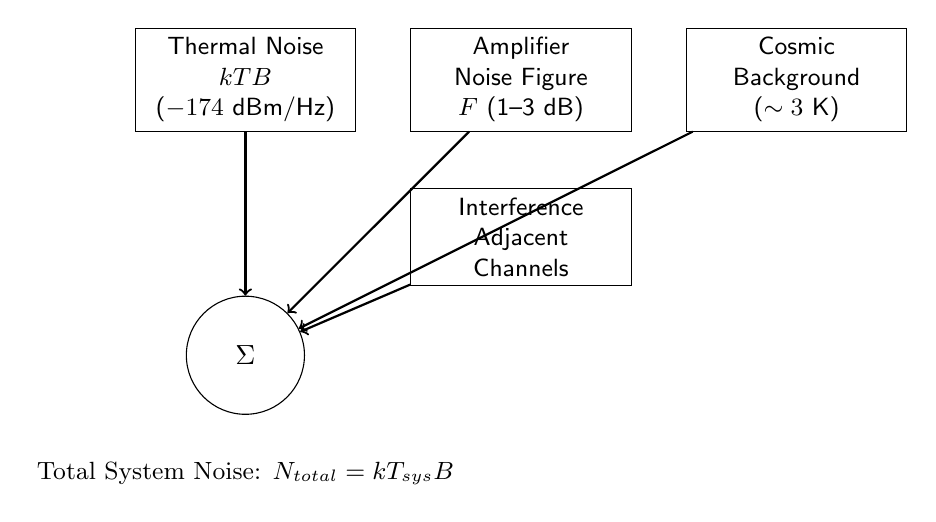
\begin{tikzpicture}[
  node distance=2cm,
  source/.style={rectangle, draw, minimum width=2.8cm, minimum height=1cm, font=\sffamily\small, align=center}
]

\node[source] (thermal) {Thermal Noise\\$kTB$\\($-174$ dBm/Hz)};
\node[source, right of=thermal, node distance=3.5cm] (amp) {Amplifier\\Noise Figure\\$F$ (1--3 dB)};
\node[source, right of=amp, node distance=3.5cm] (cosmic) {Cosmic\\Background\\($\sim 3$ K)};
\node[source, below of=amp, node distance=2cm] (interf) {Interference\\Adjacent\\Channels};

\node[draw, circle, below of=thermal, node distance=3.5cm, minimum size=1.5cm] (sum) {$\Sigma$};

\draw[->,thick] (thermal) -- (sum);
\draw[->,thick] (amp) -- (sum);
\draw[->,thick] (cosmic) -- (sum);
\draw[->,thick] (interf) -- (sum);

\node[below of=sum, node distance=1.5cm, font=\small] (total) {Total System Noise: $N_{\text{total}} = kT_{\text{sys}}B$};

\end{tikzpicture}
\end{center}

The total system noise temperature combines all sources:
\begin{equation}
T_{\text{sys}} = T_{\text{antenna}} + T_{\text{LNA}}(F-1) + T_{\text{cosmic}} + T_{\text{interference}}
\end{equation}
where:
\begin{itemize}
\item $T_{\text{antenna}}$ = antenna noise temperature (K)
\item $T_{\text{LNA}}$ = LNA physical temperature (K)
\item $F$ = LNA noise figure (linear)
\item $T_{\text{cosmic}}$ = cosmic background (typically 3 K)
\item $T_{\text{interference}}$ = equivalent temperature from interference (K)
\end{itemize}

\subsubsection{Mathematical Model}\label{mathematical-model-1}

The received signal in an AWGN channel is:
\begin{equation}
r(t) = \frac{s(t)}{L} + n(t)
\end{equation}
where:
\begin{itemize}
\item $r(t)$ = received signal (volts)
\item $s(t)$ = transmitted signal (volts)
\item $L$ = link loss factor (dimensionless)
\item $n(t)$ = additive white Gaussian noise (volts)
\end{itemize}

The noise power is independent of signal power:
\begin{equation}
N = kTB
\end{equation}
where:
\begin{itemize}
\item $k = 1.38 \times 10^{-23}$ J/K = Boltzmann constant
\item $T$ = system noise temperature (kelvin)
\item $B$ = bandwidth (Hz)
\item $N$ = noise power (watts)
\end{itemize}

\subsection{Combined Channel Model}\label{combined-channel-model}

The complete channel model applies both link loss and noise sequentially:

\begin{center}
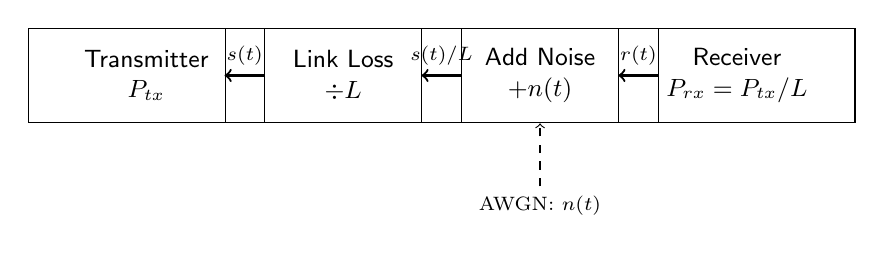
\begin{tikzpicture}[
  node distance=2.5cm,
  block/.style={rectangle, draw, minimum width=3cm, minimum height=1.2cm, font=\sffamily\small, align=center}
]

\node[block] (tx) {Transmitter\\$P_{\text{tx}}$};
\node[block, right of=tx] (loss) {Link Loss\\$\div L$};
\node[block, right of=loss] (noise) {Add Noise\\$+ n(t)$};
\node[block, right of=noise] (rx) {Receiver\\$P_{\text{rx}} = P_{\text{tx}}/L$};

\draw[->,thick] (tx) -- node[above,font=\scriptsize] {$s(t)$} (loss);
\draw[->,thick] (loss) -- node[above,font=\scriptsize] {$s(t)/L$} (noise);
\draw[->,thick] (noise) -- node[above,font=\scriptsize] {$r(t)$} (rx);

\draw[->,dashed] (noise.south) ++ (0,-0.8) node[below,font=\scriptsize] {AWGN: $n(t)$} -- (noise.south);

\end{tikzpicture}
\end{center}

\textbf{Processing steps:}
\begin{enumerate}
\item \textbf{Transmit Signal}: Power $= P_{\text{tx}}$
\item \textbf{Apply Link Loss}: Power reduced to $P_{\text{tx}} / L$ or $P_{\text{tx}} - L_{\text{dB}}$ in dB
\item \textbf{Add AWGN}: Noise power $N = kTB$ (independent of signal)
\item \textbf{Received Signal}: Attenuated signal plus noise: $r(t) = s(t)/L + n(t)$
\end{enumerate}

The signal-to-noise ratio at the receiver is:
\begin{equation}
\text{SNR} = \frac{P_{\text{tx}}/L}{N} = \frac{P_{\text{tx}}}{LN}
\end{equation}
where:
\begin{itemize}
\item SNR = signal-to-noise ratio (dimensionless)
\item $P_{\text{tx}}/L$ = received signal power after link loss
\item $N$ = noise power
\end{itemize}

\subsection{Why Both Matter}\label{why-both-matter}

\subsubsection{Link Loss Affects Signal Power}\label{link-loss-affects-signal-power}

\begin{itemize}
\item High link loss (100+ dB) is typical in many systems
\item Reduces signal level but doesn't add randomness
\item Can be compensated with amplification (but amplifies noise too!)
\end{itemize}

\subsubsection{Noise Affects Signal Quality (SNR)}\label{noise-affects-signal-quality-snr}

\begin{itemize}
\item Adds random errors that can't be predicted
\item Sets the fundamental limit on achievable BER
\item Can be improved with processing gain, error correction
\end{itemize}

\begin{calloutbox}{Physical Interpretation}
\textbf{Link loss} is like speaking into a megaphone facing away---your voice reaches far but is very quiet. \textbf{Noise} is like the background chatter in a crowded room---it doesn't affect your voice volume, but makes it harder to hear.

In communication systems:
\begin{itemize}
\item \textbf{Link loss} scales the signal: $s(t) \rightarrow s(t)/L$
\item \textbf{Noise} adds interference: $s(t)/L \rightarrow s(t)/L + n(t)$
\item \textbf{SNR combines both}: $\text{SNR} = \frac{P_{\text{signal}}/L}{N}$
\end{itemize}
\end{calloutbox}

\section{Performance Analysis}

\subsection{Link Budget and SNR}\label{link-budget-and-snr}

The combination of link loss and noise determines receiver performance. The received signal power is:
\begin{equation}
P_{\text{rx}} [\text{dBm}] = P_{\text{tx}} [\text{dBm}] - L_{\text{dB}}
\end{equation}

The thermal noise power is:
\begin{equation}
N [\text{dBm}] = 10\log_{10}(kTB) + 30
\end{equation}
where the $+30$ converts watts to dBm.

The signal-to-noise ratio in dB is:
\begin{equation}
\text{SNR} [\text{dB}] = P_{\text{rx}} [\text{dBm}] - N [\text{dBm}]
\end{equation}
\begin{equation}
\text{SNR} [\text{dB}] = P_{\text{tx}} [\text{dBm}] - L_{\text{dB}} - 10\log_{10}(kTB) - 30
\end{equation}

\subsection{Link Performance Examples}

\subsubsection{Example 1: Good Link}\label{example-1-good-link}

\begin{itemize}
\item Transmit power: $P_{\text{tx}} = +30$ dBm
\item Link loss: $L_{\text{dB}} = 100$ dB
\item Received signal: $P_{\text{rx}} = +30 - 100 = \textbf{-70}$ \textbf{dBm}
\item Noise floor: $N = -90$ dBm
\item \textbf{Resulting SNR: $-70 - (-90) = 20$ dB} --- Excellent!
\end{itemize}

\subsubsection{Example 2: Challenging Link}\label{example-2-challenging-link}

\begin{itemize}
\item Transmit power: $P_{\text{tx}} = +30$ dBm
\item Link loss: $L_{\text{dB}} = 120$ dB
\item Received signal: $P_{\text{rx}} = +30 - 120 = \textbf{-90}$ \textbf{dBm}
\item Noise floor: $N = -90$ dBm
\item \textbf{Resulting SNR: $-90 - (-90) = 0$ dB} --- Very challenging!
\end{itemize}

\begin{center}
\begin{tabular}{@{}lrrr@{}}
\toprule
\textbf{Parameter} & \textbf{Example 1} & \textbf{Example 2} & \textbf{Units} \\
\midrule
TX Power & $+30$ & $+30$ & dBm \\
Link Loss & $100$ & $120$ & dB \\
RX Signal & $-70$ & $-90$ & dBm \\
Noise Floor & $-90$ & $-90$ & dBm \\
\textbf{SNR} & \textbf{$20$} & \textbf{$0$} & \textbf{dB} \\
\textbf{Link Quality} & \textbf{Good} & \textbf{Marginal} & --- \\
\bottomrule
\end{tabular}
\end{center}

\section{Worked Example: Satellite Downlink}

\textbf{Problem:} Calculate the received signal power and SNR for a geostationary satellite downlink.

\textbf{Given Parameters:}

\begin{tabular}{@{}ll@{}}
Satellite TX power & $P_{\text{tx}} = 50$ W = $+47$ dBm \\
TX antenna gain & $G_{\text{tx}} = 30$ dBi \\
Distance & $d = 36{,}000$ km (GEO orbit) \\
Frequency & $f = 12$ GHz (Ku-band) \\
RX antenna gain & $G_{\text{rx}} = 45$ dBi (1.2 m dish) \\
System noise temp & $T_s = 100$ K \\
Bandwidth & $B = 10$ MHz \\
\end{tabular}

\textbf{Solution:}

\textbf{Step 1:} Calculate free-space path loss using the Friis equation:
\begin{equation}
\text{FSPL} [\text{dB}] = 20\log_{10}(d_{\text{km}}) + 20\log_{10}(f_{\text{MHz}}) + 32.45
\end{equation}
\begin{equation}
\text{FSPL} = 20\log_{10}(36{,}000) + 20\log_{10}(12{,}000) + 32.45 = 205.5\ \text{dB}
\end{equation}

\textbf{Step 2:} Calculate received signal power:
\begin{equation}
P_{\text{rx}} [\text{dBm}] = P_{\text{tx}} + G_{\text{tx}} + G_{\text{rx}} - \text{FSPL}
\end{equation}
\begin{equation}
P_{\text{rx}} = 47 + 30 + 45 - 205.5 = -83.5\ \text{dBm}
\end{equation}

\textbf{Step 3:} Calculate thermal noise power:
\begin{equation}
N [\text{W}] = kTB = (1.38 \times 10^{-23})(100)(10 \times 10^6) = 1.38 \times 10^{-14}\ \text{W}
\end{equation}
\begin{equation}
N [\text{dBm}] = 10\log_{10}(1.38 \times 10^{-14} / 10^{-3}) = -108.6\ \text{dBm}
\end{equation}

\textbf{Step 4:} Calculate SNR:
\begin{equation}
\text{SNR} [\text{dB}] = P_{\text{rx}} - N = -83.5 - (-108.6) = 25.1\ \text{dB}
\end{equation}

\begin{calloutbox}[colback=black!8!white,colframe=black]{Link Budget Summary}
\begin{tabular}{@{}lr@{}}
\toprule
\textbf{Parameter} & \textbf{Value} \\
\midrule
TX Power & $+47$ dBm \\
TX Antenna Gain & $+30$ dBi \\
Free-Space Path Loss & $-205.5$ dB \\
RX Antenna Gain & $+45$ dBi \\
\midrule
\textbf{Received Signal Power} & \textbf{$-83.5$ dBm} \\
Noise Power & $-108.6$ dBm \\
\midrule
\textbf{SNR} & \textbf{$25.1$ dB} \\
\textbf{Total Link Loss} & \textbf{$130.5$ dB} \\
\bottomrule
\end{tabular}

\textbf{Result:} Link closes with 25.1 dB SNR. This comfortable margin accommodates rain fade (5--10 dB at Ku-band), implementation losses (2--3 dB), and pointing errors (1--2 dB).
\end{calloutbox}

\section{Applications}

\subsection{Satellite Communications}

Satellite links face extreme path loss (150--210 dB) due to long distances:
\begin{itemize}
\item \textbf{Challenge}: Signal arrives incredibly weak at receiver
\item \textbf{Solution}: High-gain antennas (30--50 dBi) and low-noise amplifiers
\item \textbf{Example}: GPS satellites transmit 50 W, receive $-130$ dBm on Earth
\item \textbf{Trade-off}: Larger antennas increase gain but reduce portability
\end{itemize}

\subsection{Cellular Networks}

Mobile phones must overcome variable path loss and interference:
\begin{itemize}
\item \textbf{Challenge}: Path loss varies with distance, buildings, weather
\item \textbf{Solution}: Adaptive power control, cell handover, frequency reuse
\item \textbf{Example}: Urban cell tower covers 500 m (80--100 dB path loss)
\item \textbf{Trade-off}: More transmit power increases range but drains battery
\end{itemize}

\subsection{Deep-Space Missions}

Voyager probes face record path loss (310+ dB at 24 billion km):
\begin{itemize}
\item \textbf{Challenge}: Weakest signals ever detected by human receivers
\item \textbf{Solution}: 70 m Deep Space Network dishes (74 dBi), FEC coding
\item \textbf{Example}: Voyager 1 transmits 23 W, received at $-196$ dBm
\item \textbf{Trade-off}: Massive ground infrastructure required (cost, complexity)
\end{itemize}

\subsection{Wireless LANs (WiFi)}

WiFi operates in crowded spectrum with moderate path loss:
\begin{itemize}
\item \textbf{Challenge}: High noise from interference (microwaves, Bluetooth)
\item \textbf{Solution}: Spread spectrum, adaptive rate control, multiple antennas
\item \textbf{Example}: 100 mW router at 50 m has 70 dB path loss
\item \textbf{Trade-off}: Higher data rates require better SNR (shorter range)
\end{itemize}

\subsection{Key Design Insight}

\begin{center}
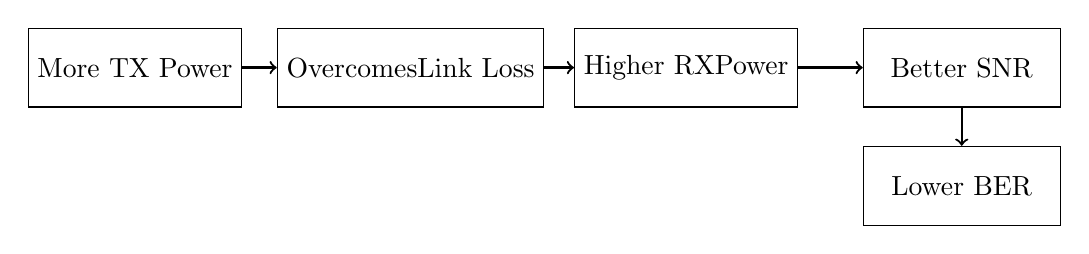
\begin{tikzpicture}[node distance=2cm]
\node (tx) [draw, rectangle, minimum width=2.5cm, minimum height=1cm] {More TX Power};
\node (loss) [draw, rectangle, right of=tx, node distance=3.5cm, minimum width=2.5cm, minimum height=1cm] {Overcomes\\Link Loss};
\node (rx) [draw, rectangle, right of=loss, node distance=3.5cm, minimum width=2.5cm, minimum height=1cm] {Higher RX\\Power};
\node (snr) [draw, rectangle, right of=rx, node distance=3.5cm, minimum width=2.5cm, minimum height=1cm] {Better SNR};
\node (ber) [draw, rectangle, below of=snr, node distance=1.5cm, minimum width=2.5cm, minimum height=1cm] {Lower BER};

\draw[->,thick] (tx) -- (loss);
\draw[->,thick] (loss) -- (rx);
\draw[->,thick] (rx) -- (snr);
\draw[->,thick] (snr) -- (ber);
\end{tikzpicture}
\end{center}

\textbf{Practical limits:}
\begin{itemize}
\item \textbf{Transmitter power}: Battery life, regulatory limits, heat dissipation
\item \textbf{Receiver sensitivity}: Thermal noise floor ($kTB$), amplifier noise figure
\item \textbf{Cost and complexity}: High-gain antennas, low-noise amplifiers
\end{itemize}

\section{Summary}

\begin{center}
\begin{tabular}{@{}lll@{}}
\toprule
\textbf{Aspect} & \textbf{Link Loss} & \textbf{Noise} \\
\midrule
Nature & Deterministic & Random \\
Effect & Attenuates signal & Adds interference \\
Scaling & Multiplicative ($\div L$) & Additive ($+ n(t)$) \\
Predictable? & Yes & No \\
Time-varying? & No (fixed path) & Yes (stochastic) \\
dB calculation & Subtraction & N/A (separate) \\
Mitigation & Higher TX power, gain & FEC, filtering, gain \\
Typical value & 60--210 dB & $-90$ to $-110$ dBm \\
\bottomrule
\end{tabular}
\end{center}

\begin{keyconcept}
\textbf{Link loss weakens the signal deterministically.} \textbf{Noise adds random interference.} Both combine to determine the SNR, which governs the bit error rate and system reliability. Understanding this distinction is essential for link budget analysis and system design.
\end{keyconcept}

\begin{warningbox}
\textbf{Common Misconception:} Amplifying a weak signal does NOT improve SNR if done after noise is added. The amplifier boosts both signal and noise equally. Low-noise amplifiers (LNAs) must be placed \textbf{immediately after the antenna} to minimize noise figure.
\end{warningbox}

\section{Further Reading}

\begin{itemize}
\item \textbf{Chapter \ref{ch:snr}:} Signal-to-Noise Ratio (SNR) --- The quality metric
\item \textbf{Chapter \ref{ch:awgn}:} Additive White Gaussian Noise (AWGN) --- The noise model
\item \textbf{Chapter \ref{ch:link-budget}:} Complete Link Budget Analysis --- Calculating system performance
\item \textbf{Chapter \ref{ch:energy-ratios}:} Energy Ratios ($E_s/N_0$ and $E_b/N_0$) --- Energy-based metrics
\item \textbf{Chapter \ref{ch:fspl}:} Free-Space Path Loss (FSPL) --- Distance-dependent attenuation
\item \textbf{Chapter \ref{ch:channel-models}:} Channel Models (Rayleigh \& Rician) --- Fading channels
\end{itemize}
